\documentclass[11pt]{report}
\usepackage[utf8]{inputenc}
\usepackage[english]{babel}
\usepackage{fancyhdr}
\usepackage[final]{pdfpages}
\setcounter{secnumdepth}{-1}
\usepackage{amsfonts}
\usepackage{float}
\pagestyle{fancy}
\usepackage{url}
\usepackage{graphicx}
\usepackage{fancyvrb}
\usepackage{alltt}
\usepackage{graphicx}
\usepackage{caption}
\usepackage{subcaption}
\usepackage{amsmath}
\usepackage{xr}
\usepackage{amssymb}
\usepackage{courier}
\nonstopmode
\pagestyle{fancy}
\lhead{Nikolaj Friis Østergaard - ltm741}
\rhead{\today}
\newcommand{\then}{\rightarrow}
\DeclareMathOperator*{\Bigcdot}{\scalerel*{\cdot}{\bigodot}}
\begin{document}
\section{1 Histogram-based processing}
\subsection{1.1}
TODO
\subsection{1.2}
If the image is normalized to have values in the range [0,1], then the PDF of a constant image is just the normalized histogram. The CDF is just
$$
y(x_k) = \sum_{j=0}^{k}p_x(x_k)
$$
The k'th entry is the sum of all previous entries.
For a constant PDF the CDF will just be a monotonically increasing, each step incremented by the same constant value.
\subsection{1.3}


\subsection{1.4}
\subsection{1.5}
Generally no, given an image transformed by a CDF, we have no way of knowing which intensities matched to which acummulated intensities.

\subsection{1.6}





\section{2 Image filtering and enhancement}

\subsection{2.1}
NOUSE
\begin{align*}
f(x,y) = \sum_{i = I_{min}}^{I_{max}}\sum_{j = J_{min}}^{J_{max}}{w(i,j)I(x+i, y+j)}
\end{align*}
The approximation for the x value uses the difference between the pixel before and the pixel after, normalized by dividing by 2. The y value is calculated the same way. This result in the kernel:
$$
Kernel =
\begin{matrix}
  0 & -0.5 & 0 \\
  -0.5 & 0 & 0.5 \\
  0 & 0.5 & 0
 \end{matrix}
$
imfilter uses correlation and convolution, uses convolution. They are almost the same, but convolution flips the kernel, on both axis. For kernels like gaussian, which are symetrical around the center, it does not matter which we choose to use.

\subsection{2.2}

The kernel in 4.5.2.1 shows the kernel in for the x derivative, and thus these will be used for discussion. Instead of just looking at the pixel to the right and the left, we also use the information about the row above and below. By using the row above and below, we don't interpret a single noise pixel as being part of and edge, since the pixels below and above does not indicate that there is a continiued edge. This makes noise get lower values then real edge, which spanned multiple rows. The same logic is applied for the y derivative, where we look at the derivatives and both sides. Sobel weigh the current rows pixels heigher the the ones below and above. Were Prewitt weigh them equally.



\subsection{2.3}
blue is median filter, red is mean filter
TODO talk about image

\begin{figure}[!ht]
    \centering
    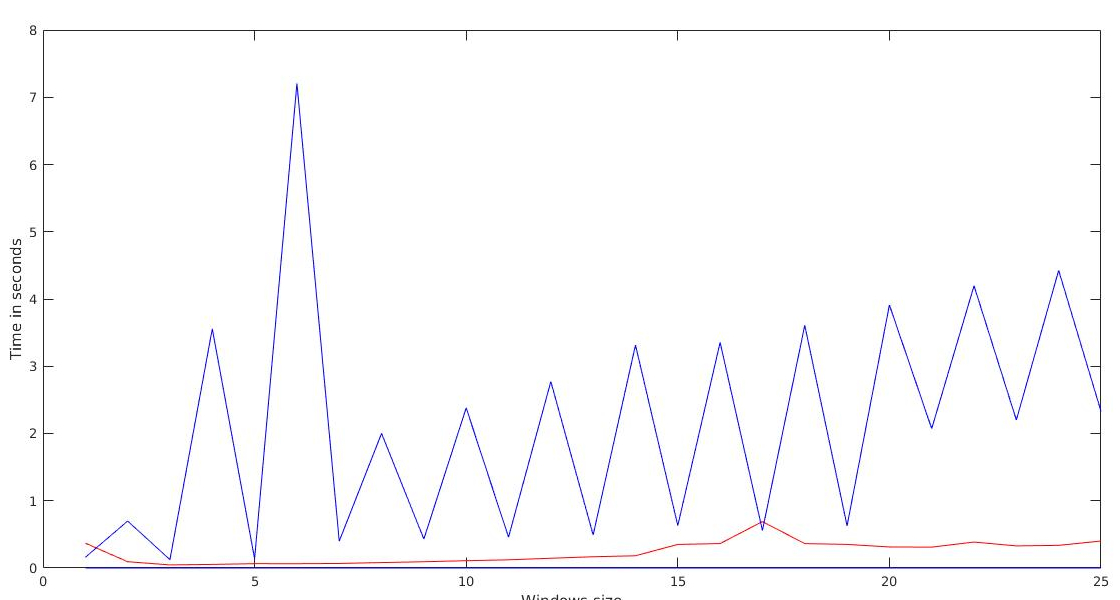
\includegraphics[width=1\textwidth]{fig23.jpg}
    \caption{9 Images with inceasing windows size starting at 3 ending at 19.}
    \label{fig:2_3}
\end{figure}

\subsection{2.4}
Filtered with gaussian kernel where $\sigma = 5$, in in the range 3:19, with increments og 2, to keep the kernel diameter odd

TODO talk about image
\begin{figure}[!ht]
    \centering
    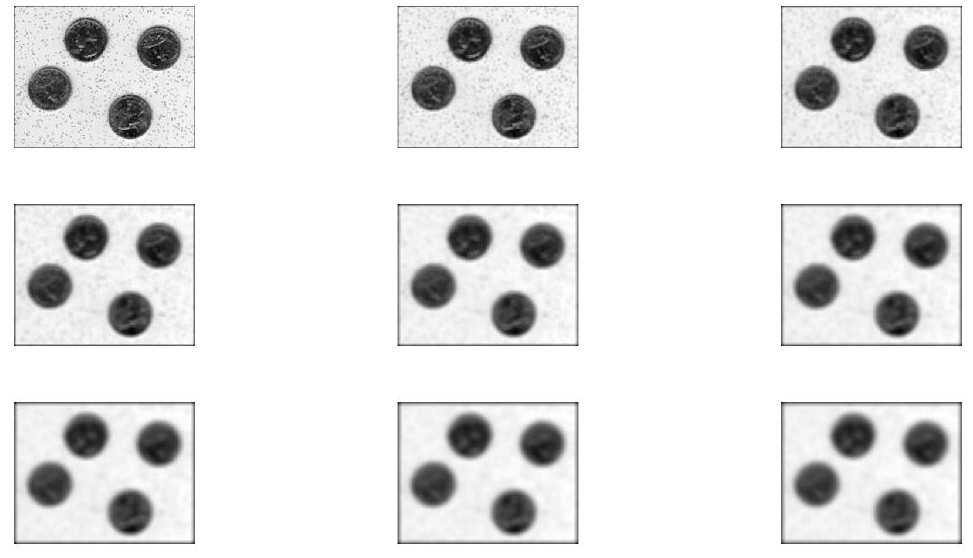
\includegraphics[width=1\textwidth]{fig24.jpg}
    \caption{9 Images with inceasing windows size starting at 3 ending at 19.}
    \label{fig:2_4}
\end{figure}

At some point the windows is so big, that the values furthest away from the center are so small, that their weight is neglectable, thus increasing the windows size show no notacible difference.

\subsection{2.5}

Figure \reg{fig:2_5} show the cameraman filter with a gaussian filter, with increasing $\sigma$ starting at 3 and ending at 19, in incremental steps of 2. The windows size N is 3*sigma + 1, and then rounding up to nearest odd integer. What we can see TODO
\begin{figure}[!ht]
    \centering
    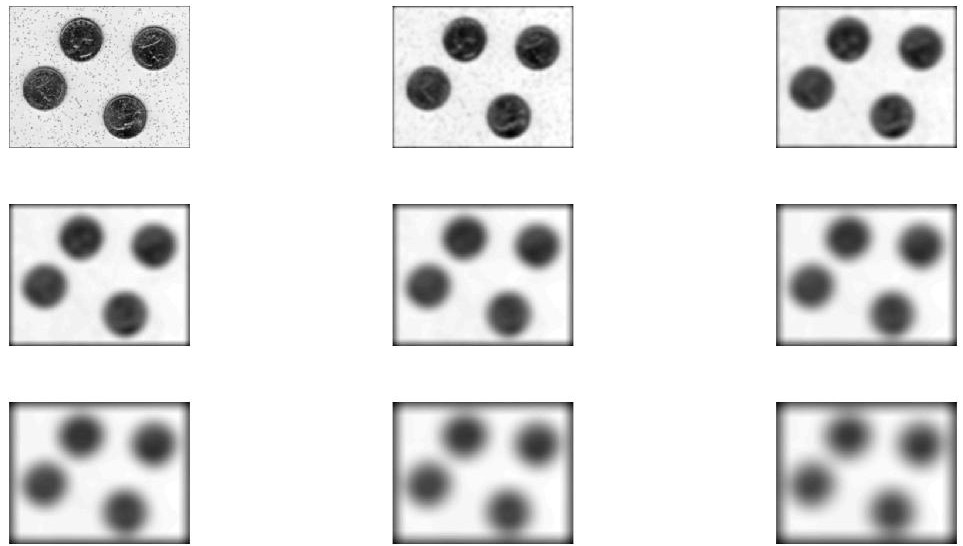
\includegraphics[width=1\textwidth]{fig25.jpg}
    \caption{9 Images with inceasing windows size starting at 3 ending at 19.}
    \label{fig:2_5}
\end{figure}

\section{3 Bonus question}


\end{document}
